%%%%%%%%%%%%%%%%%%%%%%%% ExtendedAbstract.tex %%%%%%%%%%%%%%%%%%%%%%%%
%                                                                    %
%  Template for the 10-page extended abstract to be submitted for    %
%  the MSc degree conferral at Instituto Superior Tecnico.           %
%                                                                    %
%  Author:                                                           %
%                                                                    %
%       Andre C. Marta                                               %
%       Area Cientifica de Mecanica Aplicada e Aeroespacial          %
%       Departamento de Engenharia Mecanica                          %
%       Instituto Superior Tecnico                                   %
%       Av. Rovisco Pais                                             %
%       1049-001 Lisboa                                              %
%       Portugal                                                     %
%       Tel: +351 21 841 9466                                        %
%                        3466 (extension)                            %
%       Email: andre.marta@ist.utl.pt                                %
%                                                                    %
%  Created:       Dec  2, 2011                                       %
%  Last Modified: Dec 27, 2011                                       %
%%%%%%%%%%%%%%%%%%%%%%%%%%%%%%%%%%%%%%%%%%%%%%%%%%%%%%%%%%%%%%%%%%%%%%
% This document uses the LaTeX class file "article.cls"              %
%%%%%%%%%%%%%%%%%%%%%%%%%%%%%%%%%%%%%%%%%%%%%%%%%%%%%%%%%%%%%%%%%%%%%%
\documentclass[a4paper, twocolumn]{article}

%%%%%%%%%%%%%%%%%%%%%%%%%%%%%%%%%%%%%%%%%%%%%%%%%%%%%%%%%%%%%%%%%%%%%%
% Document preamble
%%%%%%%%%%%%%%%%%%%%%%%%%%%%%%%%%%%%%%%%%%%%%%%%%%%%%%%%%%%%%%%%%%%%%%

%% Builds upon the graphics  package, providing a key-value interface
%% for optional arguments to the \includegraphics command that go far
%% beyone what the graphics package offers.
%% http://www.ctan.org/tex-archive/help/Catalogue/entries/graphicx.html
%% if you use PostScript figures in your article
%% use the graphics package for simple commands
%% \usepackage{graphics}
%% or use the graphicx package for more complicated commands
%% \usepackage{graphicx}
%% or use the epsfig package if you prefer to use the old commands
%% \usepackage{epsfig}
\usepackage{graphicx} % Enhanced LaTeX Graphics
\usepackage{siunitx}

%Tipo de letra Arial
\usepackage{helvet}
\renewcommand{\familydefault}{\sfdefault}

% acentos e cedilhas
\usepackage[utf8]{inputenc}
%\usepackage[T1]{fontenc}

% Multiple figures
%\usepackage{subfigure} % subcaptions for subfigures
%\usepackage{subfigmat} % matrices of similar subfigures

\usepackage[font=footnotesize, skip = 7pt, labelfont=bf]{caption}
\usepackage[font=footnotesize]{subcaption}

% Declaring new column types
% 'dcolumn' package defines D to be a column specifier with
% three arguments: D{<sep.tex>}{<sep.dvi>}{<decimal places>}
%                  D{<sep.tex>}{<sep.dvi>}{<left digit places>.<right digit places>}
\usepackage{dcolumn}           % decimal-aligned tabular math columns
% d takes a single argument specifying the number of decimal places, e.g., d{2}
% or the number of digits to the left and right of the seperator, e.g., d{3.2}
\newcolumntype{.}   {D{.}{.}{-1}} % column alignedd on the point separator '.'
\newcolumntype{d}[1]{D{.}{.}{#1}} % column centered on the point separator '.'
\newcolumntype{e}   {D{E}{E}{-1}} % column centered on the exponent 'E'
\newcolumntype{E}[1]{D{E}{E}{#1}} % column centered on the exponent 'E'

%% American Mathematical Society (AMS) plain Tex macros
%%
%% The amsmath package is the principal package in the AMS-LaTeX distribution
%% http://www.ctan.org/tex-archive/help/Catalogue/entries/amsmath.html
\usepackage{amsmath}
\DeclareMathSizes{7}{7}{3}{3} 
\usepackage{pifont}
%%
%% The amsfonts package provides extended TeX fonts
%% http://www.ctan.org/tex-archive/help/Catalogue/entries/amsfonts.html
\usepackage{amsfonts}
%% The amssymb package provides various useful mathematical symbols
\usepackage{amssymb}
%%
%% The amsthm package provides extended theorem environments
%% http://www.ctan.org/tex-archive/help/Catalogue/entries/amsthm.html
\usepackage{amsthm}

%% Improves the interface for defining floating objects such as figures and tables.
%% The package also provides the H float modifier option of the obsolete here package.
%% http://www.ctan.org/tex-archive/help/Catalogue/entries/float.html
\usepackage{float}

%% Control sectional headers. 
%% http://www.ctan.org/tex-archive/help/Catalogue/entries/sectsty.html
\usepackage{sectsty}
%%
%% Redefine the font size of the 'section' and 'subsection' headings
\newcommand{\myFontSize}{\fontsize{9}{0}\selectfont}
\sectionfont{\myFontSize}       % 10pt, Bold face (default)
\subsectionfont{\myFontSize} % 10pt, Plain face

%% Select alternative section titles.
%% http://www.ctan.org/tex-archive/help/Catalogue/entries/titlesec.html
\usepackage{titlesec}
\usepackage{booktabs}
%\usepackage{multirow}
%\usepackage{array}
\usepackage{csquotes}% Recommended
%\usepackage[style=authoryear, backend=bibtex, doi=false,isbn=false,url=false,eprint=false,dashed=false,maxcitenames=2, maxbibnames=100]{biblatex}
%\addbibresource{library.bib}

%%
%% Left indent, before and after spacing
%% (The starred version kills the indentation of the paragraph following the title)
\titlespacing*{\section}{0pt}{10pt}{0pt}
\titlespacing*{\subsection}{0pt}{10pt}{0pt}

%% Section numbers with trailing dots. 
%% http://www.ctan.org/tex-archive/help/Catalogue/entries/secdot.html
\usepackage{secdot}
\usepackage{epstopdf}
%%
%% Also put a dot after the subsection number
\sectiondot{subsection}
%% Set a space between dot and heading text
\sectionpunct{section}{. }    % By default, \sectiondot places a \quad
\sectionpunct{subsection}{. } % after the number

% These are exact settings for a A4 page with top margin of
% 25 mm, bottom margin of 30 mm, left and right margins of 25 mm,
% printable area 242 X 160 mm.

\setlength{\topmargin}{-10.4mm}
\setlength{\headheight}{0.0mm}
\setlength{\headsep}{10.0mm}
\setlength{\textwidth}{160mm}
\setlength{\textheight}{242mm}
\setlength{\oddsidemargin}{0mm}
\setlength{\evensidemargin}{0mm}
\setlength{\marginparwidth}{0mm}
\setlength{\marginparsep}{0mm}

% New command to refer to equations as Eq.(1),Eq.(2),...
\newcommand{\eqnref}[1]{Eq.(\ref{#1})}

%%%%%%%%%%%%%%%%%%%%%%%%%%%%%%%%%%%%%%%%%%%%%%%%%%%%%%%%%%%%%%%%%%%%%%%%%%%%%%%%%%%%%%%%
% Title, authors and addresses

\title{\bfseries Ultra-Low Noise Analog Electronic Interface \\ for Early Cancer Detection}
\date{May 2023}
\author{Artur Maria Bandeira do Amaral Rafael \\ artur.rafael@tecnico.ulisboa.pt \\ \\ Instituto Superior Técnico, Lisboa, Portugal}

%%%%%%%%%%%%%%%%%%%%%%%%%%%%%%%%%%%%%%%%%%%%%%%%%%%%%%%%%%%%%%%%%%%%%%%%%%%%%%%%%%%%%%%%
\begin{document}

% Begin one column section for title and abstract
%
% http://www.faqs.org/faqs/de-tex-faq/part5/
\twocolumn[
\begin{@twocolumnfalse}
\maketitle

	%%%%%%%%%%%%%%%%%%%%%%%%%%%%%%%%%%%%%%%%%%%%%%%%%%%%%%%%%%%%%%%%%%%%%%
%     File: ExtendedAbstract_abstr.tex                               %
%     Tex Master: ExtendedAbstract.tex                               %
%                                                                    %
%     Author: Andre Calado Marta                                     %
%     Last modified : 2 Dez 2011                                     %
%%%%%%%%%%%%%%%%%%%%%%%%%%%%%%%%%%%%%%%%%%%%%%%%%%%%%%%%%%%%%%%%%%%%%%
% The abstract of should have less than 500 words.
% The keywords should be typed here (three to five keywords).
%%%%%%%%%%%%%%%%%%%%%%%%%%%%%%%%%%%%%%%%%%%%%%%%%%%%%%%%%%%%%%%%%%%%%%

%%
%% Abstract
%%
\begin{abstract}

\noindent
Flow cytometry plays a crucial role in biology and medicine by facilitating cell analysis. However, it faces significant challenges in terms of cost, integration, and portability. This work introduces a magnetic flow cytometric technique designed to address these limitations, specifically focusing on the detection and enumeration of circulating tumor cells in the bloodstream of cancer patients. The proposed system employs a microfluidic channel with integrated magnetic sensors to count tumor cells. Prior to introduction into the system, target tumor cells are bound with a magnetic cancer marker, enabling their magnetic detection within the microfluidic channel. The magnetic flow cytometer comprises three primary sections: analogue bias and amplification, analogue-to-digital conversion, and signal processing. This research centers on the analogue circuit responsible for interfacing with the magnetoresistive sensors. The primary objective of this interface is to overcome previous limitations and incorporate advanced features to facilitate comprehensive studies.
\\
%%
%% Keywords (max 5)
%%
\noindent{{\bf Keywords:}} Biomedical Analysis; Magnetic Flow Cytometry; Magnetoresistive Sensors; Ultra-Low Noise Platform; Circuit Design \\

\end{abstract}



\end{@twocolumnfalse}
]
	\section{Introduction}
\label{sec:intro}

This document highlights a work conducted at Instituto de Engenharia de Sistemas e Computadores (INESC), focusing on developing a Magnetic Flow Cytometer (MFC) system for early cancer detection \cite{JoseC_thesis, PMID24761029}. The objective is to enhance the analog front-end of the MFC, addressing its limitations and incorporating novel features to facilitate advanced studies.

The primary aim of this work is to achieve a high Signal-to-Noise Ratio (SNR) in the system by carefully managing noise sources and implementing effective noise reduction strategies. This involves optimizing the analog interface, which encompasses the electronic circuits responsible for biasing the sensors, establishing optimal electrical conditions for signal generation, and amplifying and filtering the signal prior to digitization. The platform can provide improved sensitivity and accuracy for magnetic field analysis in the cytometer system by minimising noise and ensuring a favourable SNR.

Additionally, the new platform has increased analog channels in the system, enhancing its capability for detecting circulating tumor cells responsible for tumor metastasis. The integration of microfluidics, Magnetoresistive (MR) sensors, and microelectronics allows for the precise detection and enumeration of these cells in the bloodstream of cancer patients.

The circuits in this work were designed by myself and research teams from INESC. Teams at INESC and International Iberian Nanotechnology Laboratory developed the magnetic sensors used in the cytometer system. The collaboration and expertise of everyone have resulted in robust and cutting-edge circuitry and sensor technology, ensuring a state-of-the-art platform with reliable and accurate magnetic field analysis capabilities in the MFC system.
	% A Theory section should extend, not repeat, the background to the
% article already dealt with in the Introduction and lay the
% foundation for further work.

\section{Magnetic Flow Cytometry}
\label{sec:mfc}

The MFC is a powerful tool used for characterizing immune cell phenotypes and monitoring various diseases, including solid tumors and hematological malignancies \cite{cpim.40}. In this project, MR sensors are used paired with a permanent magnet in the MFC system. To detect non-magnetic cells, magnetic markers, known as Magnetic Nano Particles (MNPs), are bonded to the analytes, generating a magnetic field near the permanent magnet.

Efficient labeling is crucial for the MFC detection system, as the signal from the MR sensors depends on the amount of MNPs on the cell's surface. The MFC system has a dynamic range, and the MR sensor response is proportional to the average fringe field generated by the MNPs. Therefore, achieving a high labeling efficiency is essential for accurate quantitative analysis.

To ensure effective labeling, specific ligand molecules \cite{Freitas2017SpintronicBF} are used to create a bridge between the magnetic particles and the cell's outer surface. The bonding process efficiency varies depending on the size of the magnetic label. Researchers have made significant efforts to choose or create the correct bead and antibody conjugates to optimize the labeling process.

Once the cells are labeled with MNPs, they are magnetized and injected into a microfluidic channel within the system. The detection mechanism in the MFC platform relies on the interaction between the tagged analytes and the MR sensors. The permanent magnet magnetizes the MNPs, attracting them closer to the sensor surface through vertical magnetophoresis. The MR sensors pick up the magnetic field \cite{DiogoC_thesis} produced by the particles, resulting in a change in resistance according to Equation \ref{eq:mr-change}.
\begin{equation}
\label{eq:mr-change}
    R_{MR}(H) = R_{NOM} + \Delta R(H) \quad [\Omega]
\end{equation}

The resistance of the MR sensors varies depending on the orientation and intensity of the magnetic field. These sensors have a fixed nominal resistance ($R_{NOM}$) and a field-dependent resistance variation ($\Delta R(H)$). The interaction between the sensors and particles produces a monocycle pulse if the excitation field is perpendicular to the particle, resulting in a specific signal pattern.
	\section{Front-End Interface}
\label{sec:fei}

This section discloses an analysis and assessment of the circuitry employed in the cytometer platform. By considering the previous platforms \cite{PMID24761029, Germano2006MICROSYSTEMFB, TIM.2013.2296417}, this study introduces innovative features to enhance the MFC system performance.

\subsection{Bias Architecture}

The MR sensors, being passive elements, require biasing to ensure accurate signal measurements. The bias architecture consists of two circuit blocks: the reference voltage and the biasing topology. The reference voltage provides stability and serves as a reference for the biasing topology, which generates and supplies a known current to the sensor. By measuring the change in voltage, it is possible to determine the magnitude and direction of the magnetic field being sensed by the sensor.

The bias topology employs a combination of a Voltage-Controlled Current Source (VCCS) circuit and an emitter degenerated current mirror. The VCCS circuit converts a reference voltage into a proportional current, while the current mirror circuit replicates or mirrors this current, ensuring its independence from the sensor. The topology can be seen in Figure \ref{fig:bias-full}.

\begin{figure}[!ht]
    \centering
    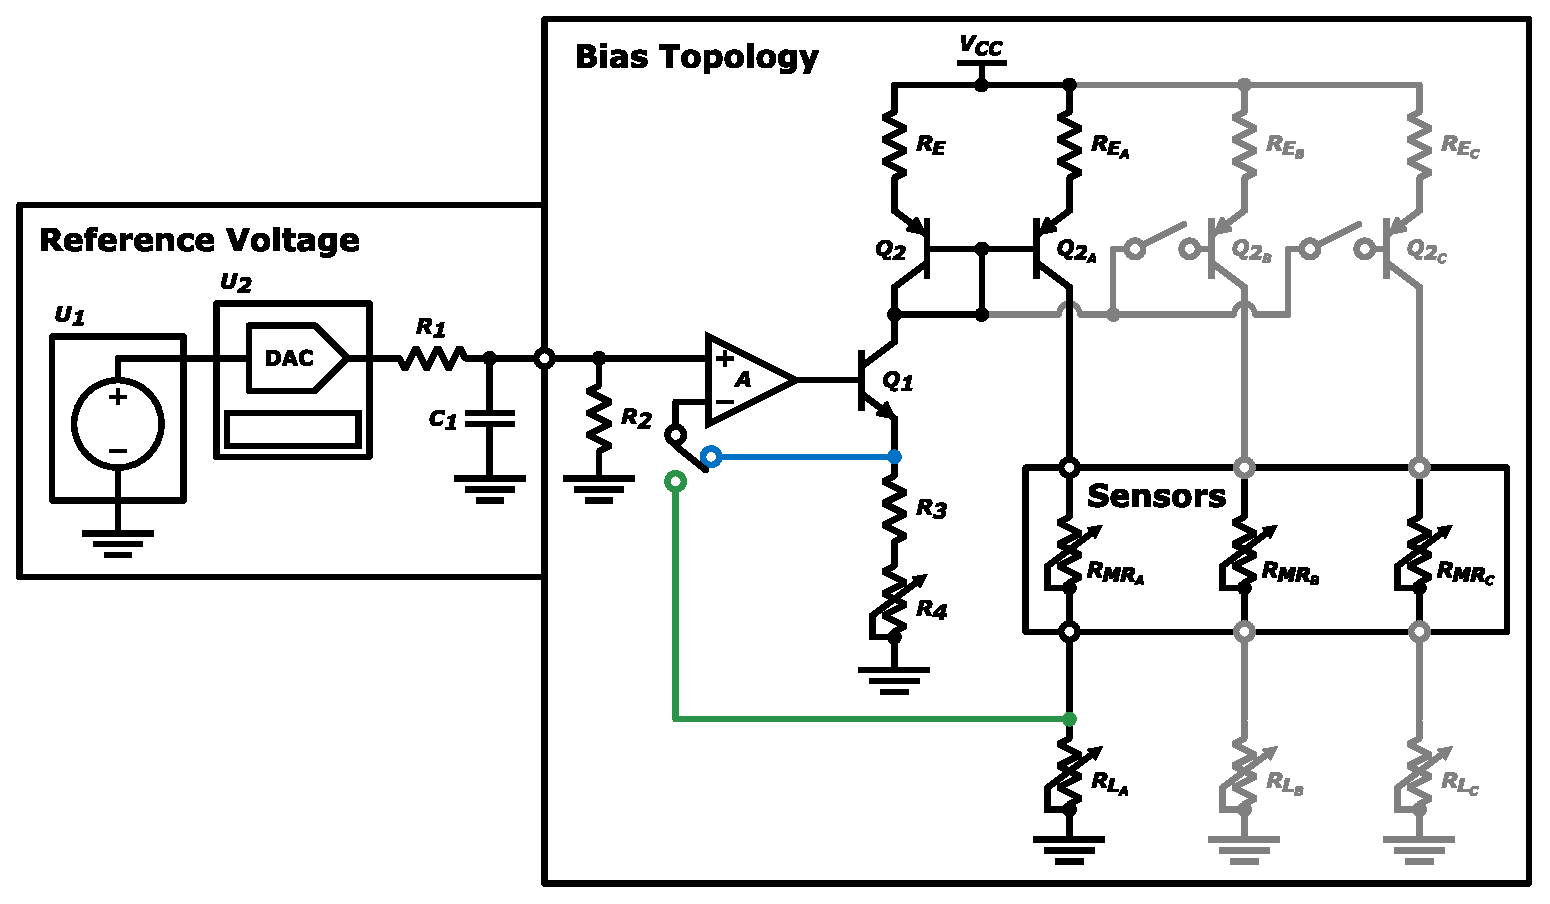
\includegraphics[width=.475\textwidth]{figs/bias_full.eps}
    \caption{Biasing architecture.}
    \label{fig:bias-full}
\end{figure}

The Figure \ref{fig:bias-full} bias circuit in the cytometer platform was designed to accommodate two different topologies: the blue line topology and the green line topology.
The blue line topology, which was used in previous versions of the cytometer, places the sensor outside the feedback loop. This topology has been proven effective and serves as the primary design choice for the bias circuit. On the other hand, the green line topology, which places the sensor inside the feedback loop, is an alternative that has not yet been validated to reduce noise. It is included in the architecture to enable further investigation and experimentation.

To achieve precise and stable biasing in electronic circuits, a voltage reference generator coupled with a digital-to-analog converter (DAC) circuit was developed (Figure \ref{fig:vref-schematic}). This approach \cite{Germano2006MICROSYSTEMFB} ensures accurate control over the output current, even in the presence of environmental factors. The DAC allows for digital adjustment of the reference voltage, providing flexibility and enabling the generation of arbitrary waveforms.

\begin{figure}[!ht]
    \centering
    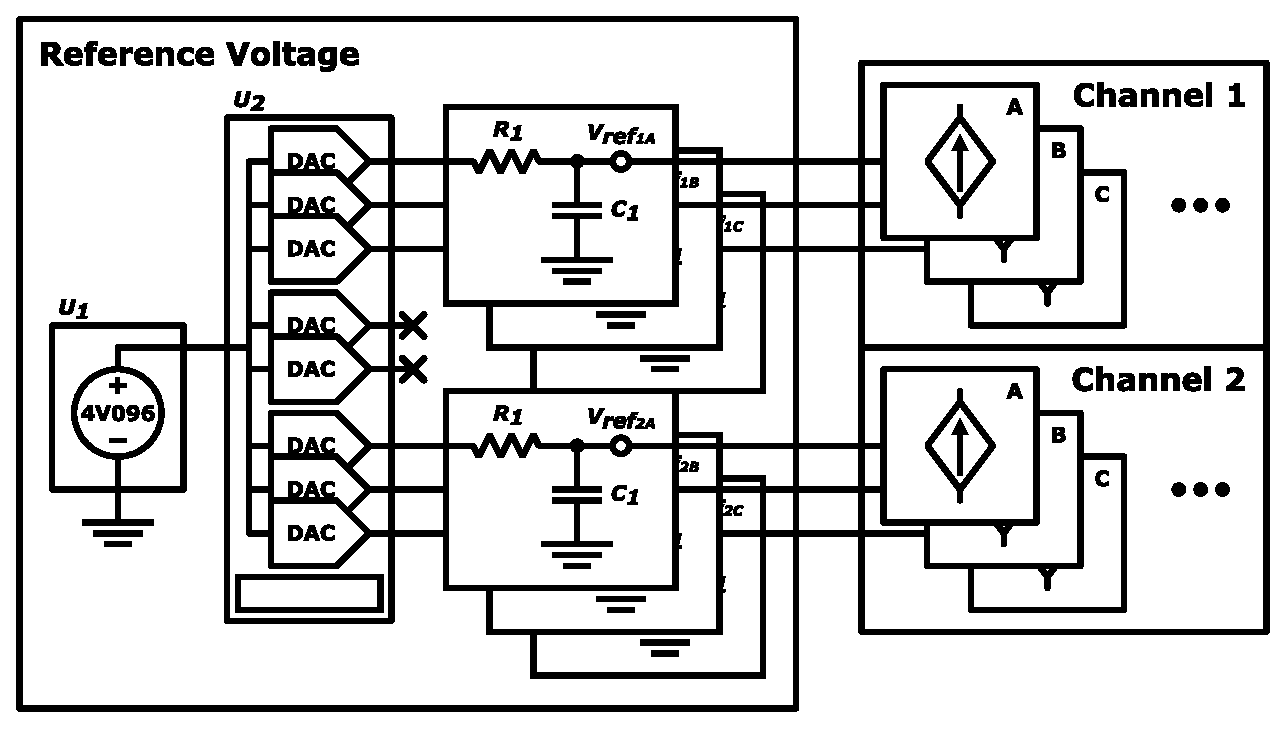
\includegraphics[width=.475\textwidth]{figs/vref.eps}
    \caption{Reference voltage schematic.}
    \label{fig:vref-schematic}
\end{figure}

The reference voltage schematic used in the interface of the cytometer platform is shown in Figure \ref{fig:vref-schematic}. Variations in the nominal resistance of the sensors may occur. To address this issue, a DAC is utilized to individually adjust the current feeding of each sensor. This allows for compensation without the need for more accurate components like precise resistors or potentiometers.

% #############################################################################
\subsection{Amplification Scheme}

In this application, magnetic particles passing through a magnetic sensor generate pulses that represent the number of analytes in the sample. The sensor signal is converted using an analog-to-digital converter (ADC) for digital processing. To ensure optimal performance and reduce quantization noise, the signal is amplified. Given that the sensor response signal is typically in the hundreds of microvolts range, the amplification scheme employed will boost the signal by a factor of 10,000.

The amplification scheme consists of two stages \cite{TIM.2013.2296417}. The first stage utilizes a differential amplifier that subtracts common voltages between input terminals, effectively reducing the impact of common noise on measurement accuracy. This stage is crucial for establishing the system's SNR. The second stage employs a non-inverting amplifier for further amplification. The circuit is completed with an anti-aliasing filter at the output. Figure \ref{fig:amp-schematic} illustrates the amplification scheme.

\begin{figure}[!ht]
    \centering
    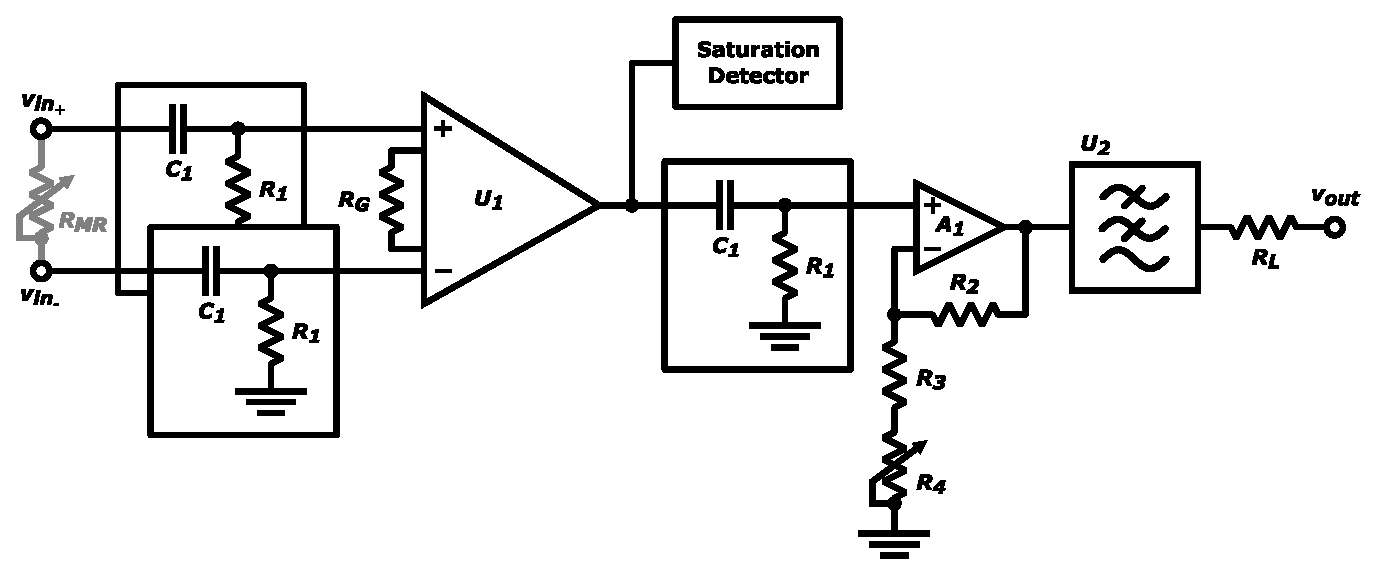
\includegraphics[width=.475\textwidth]{figs/amp.eps}
    \caption{Amplification and filtering schematic.}
    \label{fig:amp-schematic}
\end{figure}


An auxiliary circuit has been developed to address issues of signal saturation in the first stage due to noise. This circuit provides a mechanism to detect and possibly remove saturated acquired samples by alerting the user when the signal saturates. Figure \ref{fig:sat} illustrates the circuit for the "Saturation Detector" block, as shown in Figure \ref{fig:amp-schematic}. 

\begin{figure}[!ht]
    \centering
    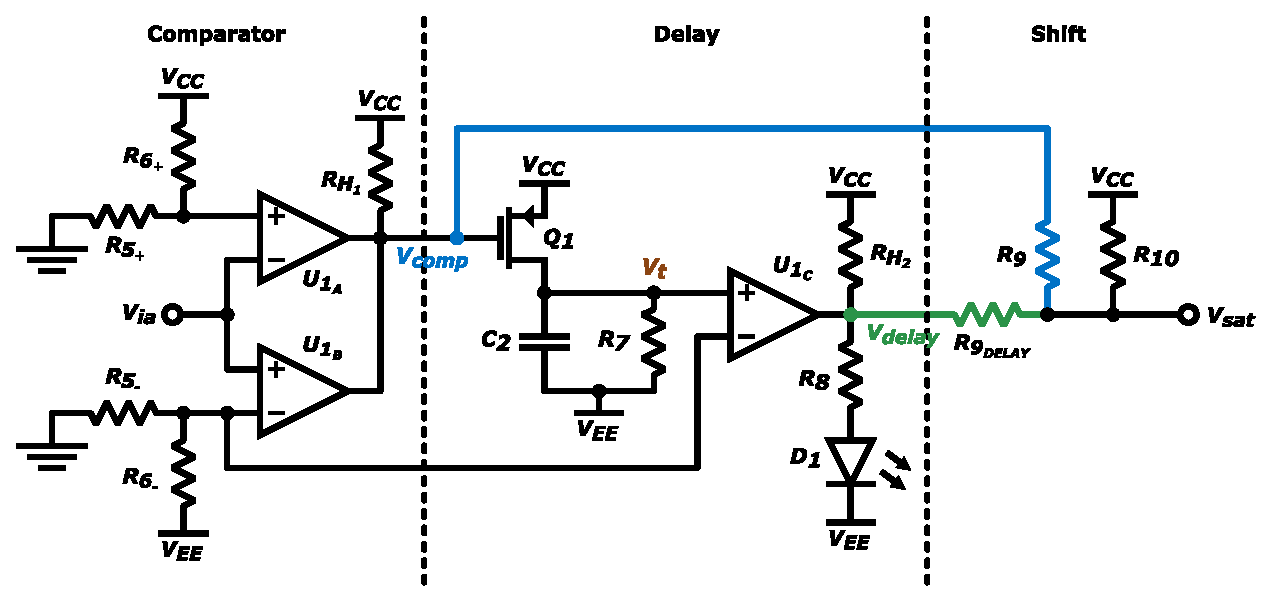
\includegraphics[width=.475\textwidth]{figs/sat.eps}
    \caption{Saturation detector circuit.}
    \label{fig:sat}
\end{figure}

The circuit in Figure \ref{fig:sat} can be divided into three segments: Comparator, Delay, and Shift. The Comparator segment is responsible for detecting when the differential amplifier saturates. The Delay segment ensures that the light-emitting diode remains on for a period of time that is noticeable to the human eye, providing a more reliable indication of saturation. Additionally, the Shift block changes the signal range. This block enables the saturated signal to be utilized in subsequent digital analysis and processing steps.
% #############################################################################

% #############################################################################
\subsection{Sensor Addressing}

The chip containing the MR sensors has been designed and manufactured at INESC, and it is connected to a custom-designed Printed Circuit Board (PCB) via wire bonding. To simplify the process of acquiring signals from the sensors, a sensor addressing module has been implemented. This module utilizes multiplexers to enable seamless switching between sensors and improve the functionality of the cytometer platform.

The implemented multiplexers enable the selection of 4 out of the 28 sensors on the chip. With 6 analog channels on the board, incorporating biasing and amplification, a total of 26 sensors can be utilized by the system. Figure \ref{fig:sensormux} shows the multiplexing circuit applied to one analog channel.

\begin{figure}[!ht]
    \centering
    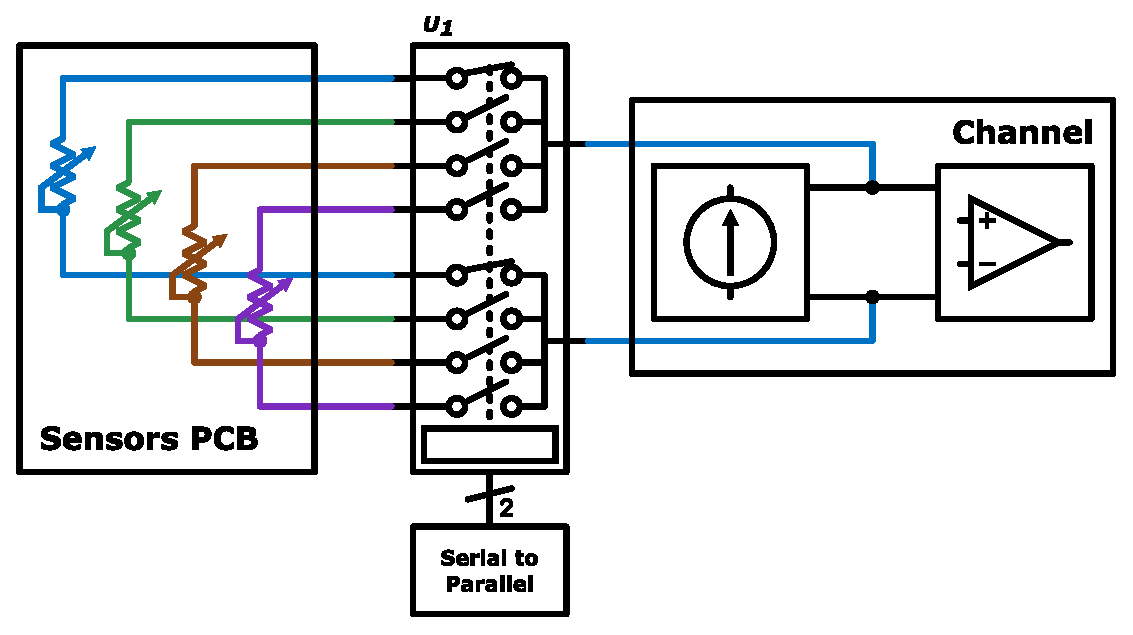
\includegraphics[width=.475\textwidth]{figs/sensormux.eps}
    \caption{Sensor addressing module.}
    \label{fig:sensormux}
\end{figure}

Figure \ref{fig:sensormux} provides a schematic diagram of the circuit used in the module and illustrates its integration into the cytometer system. The diagram shows that the first inputs of either output are selected, as indicated by the closed switch. This configuration routes the signal from the blue sensor to the output of the multiplexer, which then connects to the output of the biasing topology and the input of the amplification scheme.

To minimize the number of inputs required for the multiplexers that are using parallel communication, a circuit utilizing shift registers was developed. The Figure \ref{fig:s2p} circuit converts the parallel communication into a Serial Peripheral Interface (SPI), which reduces the number of required inputs.

\begin{figure}[!ht]
    \centering
    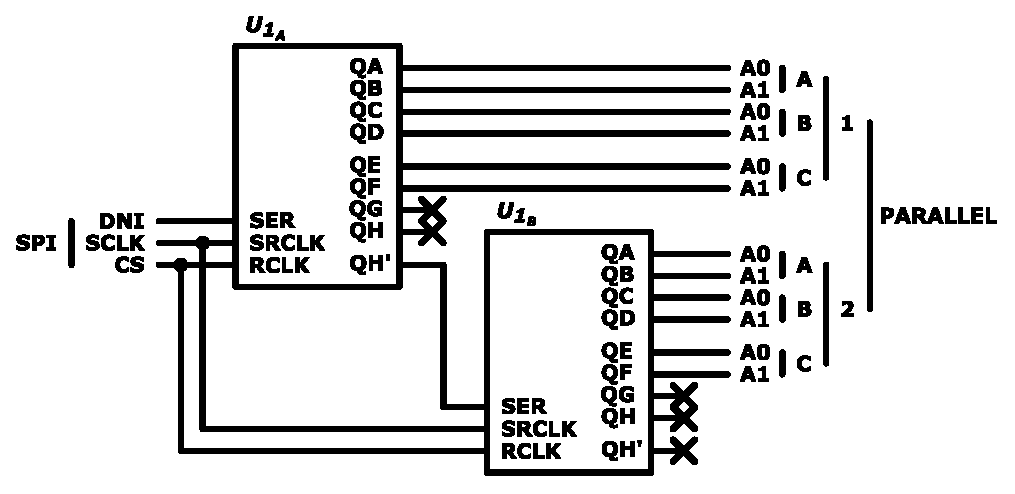
\includegraphics[width=.475\textwidth]{figs/s2p.eps}
    \caption{Serial to parallel converter circuit.}
    \label{fig:s2p}
\end{figure}

In future versions of the cytometer platform, it is recommended to use different multiplexers controlled via SPI. If such multiplexers are used, the current module converting serial communication to parallel form may become obsolete and should be removed.
% #############################################################################

% #############################################################################
\subsection{Communication Translator}

The cytometer platform includes level shifters to ensure compatibility with different controlling or data acquisition systems. These level shifters separate and convert the voltage signals to match the operating voltage of the respective devices, facilitating seamless communication and data exchange between the platform and external systems. Additionally, the platform is equipped with multiple inputs and outputs to enable efficient operation and information gathering from the board. All the signals can be found in Figure \ref{fig:level-shifters}.

The cytometer PCB was designed to connect to a Field-Programmable Gate Array (FPGA) that performs real-time Digital Signal Processing (DSP). This integration with the FPGA is expected to enhance the system's SNR and resolution. The FPGA carries out initial event detection and stores the events as a bitstream for subsequent preprocessing.

\begin{figure}[!ht]
    \centering
    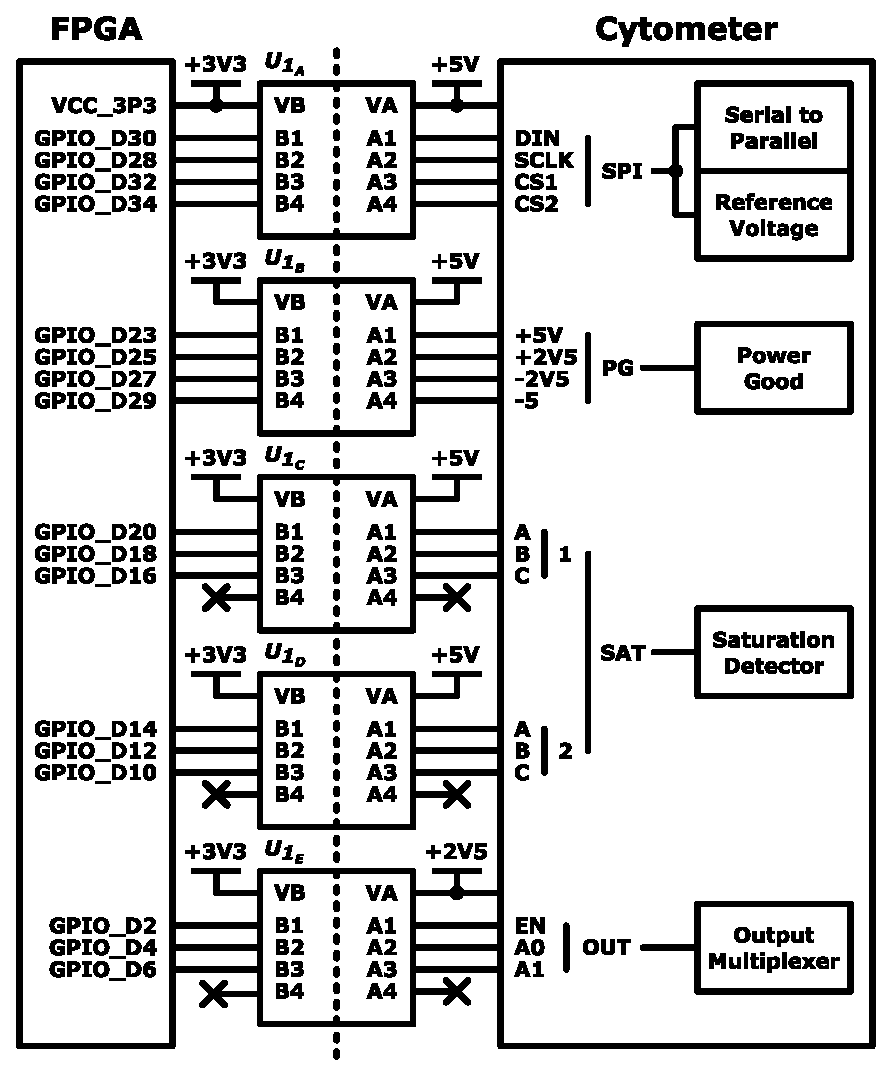
\includegraphics[width=.475\textwidth]{figs/comms.eps}
    \caption{Level shifters circuit.}
    \label{fig:level-shifters}
\end{figure}

Figure \ref{fig:level-shifters} depicts all the blocks that provide or need signals. The SPI communication protocol will be used by two circuit blocks: the serial-to-parallel block and the reference voltage block. Each block has its own chip-select signal. The serial-to-parallel block converts the serial protocol into bits that can be understood by the multiplexers in the sensor addressing circuit. The power good block, although not introduced yet, assesses whether the supply rails have sufficient voltage for the proper operation of the circuits. The FPGA can use this information to determine if the cytometer is ready to receive instructions. The saturation detector block provides information to the real-time DSP by identifying saturated signals during the amplification scheme, ensuring that such samples are not used in subsequent processing steps.
% #############################################################################

% #############################################################################
\subsection{Output Multiplexing}

To overcome the limitation of having only 2 ADCs available on the THDB-ADA acquisition board, a dedicated circuit was developed (Figure \ref{fig:outmux}) to multiplex the 6 analog channels of the cytometer platform into 2 outputs. This multiplexing circuit efficiently addresses the challenge by allowing the sharing of ADCs across multiple channels, effectively maximizing the utilization of the available resources. By multiplexing the channels, the cytometer platform can still acquire data from all 6 channels, ensuring comprehensive data collection and analysis.

\begin{figure}[!ht]
    \centering
    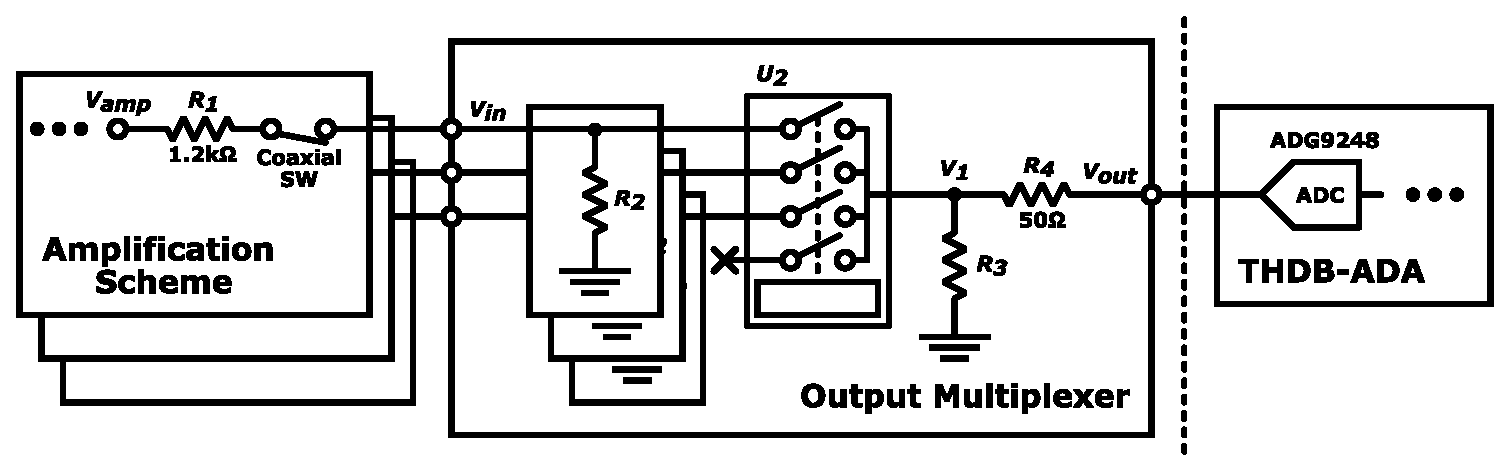
\includegraphics[width=.475\textwidth]{figs/outmux.eps}
    \caption{Output multiplexer circuit.}
    \label{fig:outmux}
\end{figure}

The circuit depicted in Figure \ref{fig:outmux} demonstrates the implementation of output multiplexing in the developed cytometer platform. Although the picture shows a single channel, it should be understood that this circuit is replicated twice to accommodate the two channels in total. To ensure maximum sampling rate of the ADCs, multiplexers with switching times lower than the sampling period were carefully selected for the purpose of channel multiplexing. If any of the inputs exceed the maximum or minimum supply voltage, the multiplexer clamps, effectively shutting down. In such cases, crosstalk may occur between the selected channel and the input signal that exceeded the supply voltage. Therefore, it is crucial for the circuit to ensure that the input signals stay within the range of $\mathrm{\pm2.5~V}$, and the output does not exceed the $\mathrm{\pm1~V}$. This limitation is necessary because the acquisition board ADCs cannot handle higher voltages, as previously specified. The voltage reduction is achieved through a two-step process using voltage dividers. This design approach ensures compatibility with the previous version of the cytometer, utilizing the same ADC and enabling broader compatibility beyond FPGA usage.

This module is designed to function independently, with inputs being connected through
SMA connectors. The amplification scheme can be detached from this circuit using the coaxial switches mentioned in the relevant section. This unique feature allows this module to be utilized as a mini-board for other applications.
% #############################################################################

% #############################################################################
\subsection{Power Supply}

Power supply is a critical aspect of electronic circuits as it enables the proper functioning of circuit components and the generation of desired electrical signals. This section explores the power circuits in detail to ensure optimal performance, reliability, and longevity of the electronic system.

The cytometer platform requires four supply rails: $\mathrm{+5~V}$, $\mathrm{+2.5~V}$, $\mathrm{-2.5~V}$, and $\mathrm{-5~V}$. To enhance flexibility, the circuit is designed to accommodate multiple power sources. Batteries offer reliability, minimal noise, and portability, making them ideal for experiments and field use. A laboratory power supply can be used as an alternative, although it may introduce higher levels of noise and reduce portability. The FPGA can also provide power, simplifying the setup process and reducing complexity. Universal Serial Bus (USB) power can also be utilized, using power banks or direct connections to a computer. Figure \ref{fig:pwr-sources} illustrates the transformation of power sources into the necessary power rails for the PCB.

\begin{figure}[!ht]
    \centering
    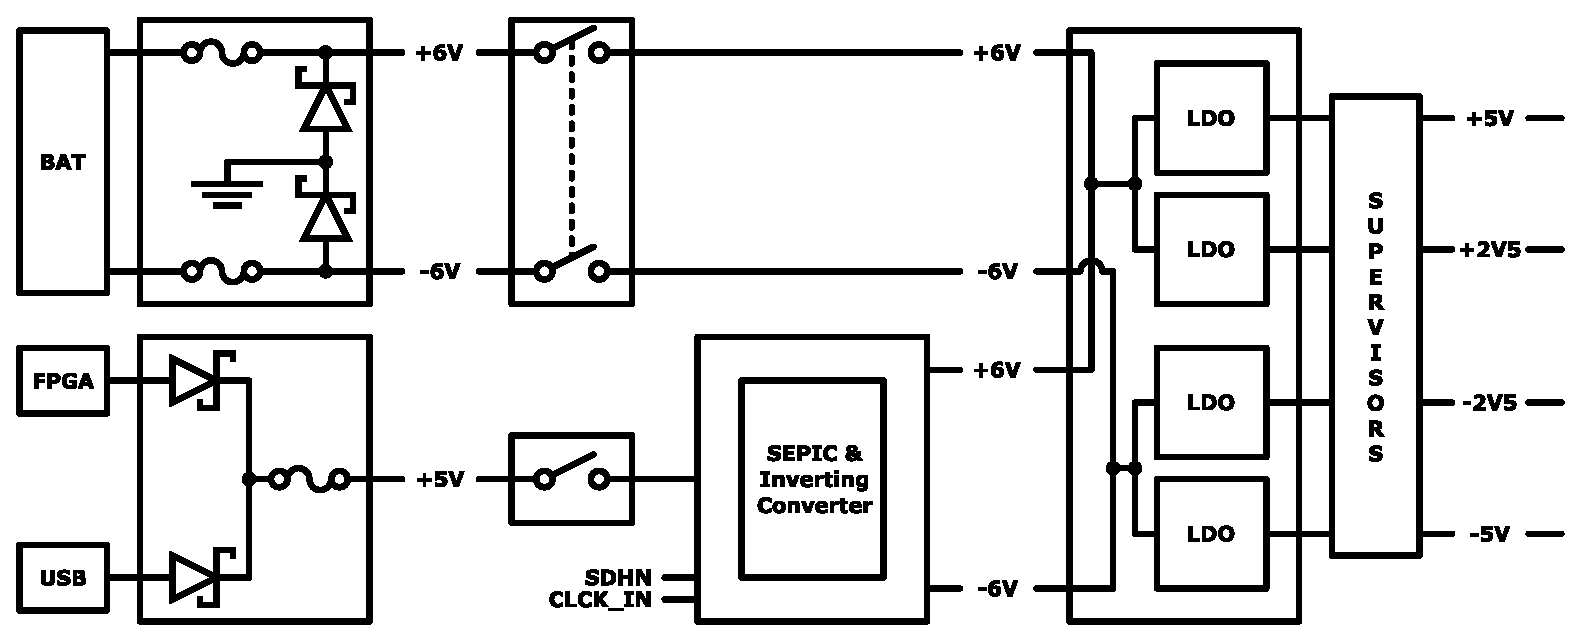
\includegraphics[width=.475\textwidth]{figs/power.eps}
    \caption{Power circuit diagram.}
    \label{fig:pwr-sources}
\end{figure}

As depicted in Figure \ref{fig:pwr-sources} the different power sources have different paths. Measures are implemented to ensure safe and efficient utilization of these power sources. A power protection circuit safeguards subsequent circuits when the battery is wrongly connected. The diodes isolates the FPGA and USB power sources to prevent current flow between them. A DC/DC converter, specifically a SEPIC and inverting circuit, boosts the signal and inverts the polarity of the rail generating $\mathrm{\pm6~V}$ rails. A Low-dropout (LDO) regulator circuit adjusts these input voltages to meet PCB requirements, providing a stable and reliable power supply. The power supervisor circuit, after the LDOs, in the cytometer platform PCB adds an extra layer of protection and user awareness, ensuring that power supply conditions are monitored and potential issues are detected in a timely manner.

By understanding and implementing these power conversion and protection mechanisms, the PCB can efficiently utilize available power sources and provide regulated voltages for proper circuit functionality. This ensures the reliable operation of the cytometer platform in various operating scenarios.
% #############################################################################


	\section{Results and Discussion}
\label{sec:res-disc}

The evaluation of noise levels and harmonic distortion is vital in assessing the performance and reliability of electronic systems. In the context of the cytometer platform, accurate measurements of noise and harmonics provide insights into the system's ability to maintain signal integrity and mitigate external disturbances. This section presents the results of comprehensive noise and harmonic measurements conducted on the platform, revealing its noise reduction capabilities and harmonic attenuation performance.

% --- Harmonics ---

Thorough testing of the cytometer platform required the inclusion of MR sensors to detect and measure changes in magnetic fields. To generate the necessary magnetic field for testing, a system comprising two coils and a driver power op-amp was utilized. The coils, arranged in a Helmholtz coil pair configuration, created a nearly uniform magnetic field, providing a controlled environment for the MR sensors. This allowed for accurate performance testing and validation of the platform's functionality.

One important performance test conducted using this system was the evaluation of harmonic distortion, depicted in Figure \ref{fig:harmonics}. Harmonics can introduce noise and distort the waveform shape, potentially compromising signal quality. Managing harmonic distortion is crucial for maintaining signal integrity in sensitive applications like the cytometer platform. 

The test involved two experiments, each utilizing a magnetic field with different frequencies. The blue trace represents the $\mathrm{1~kHz}$ frequency, while the green trace represents the $\mathrm{10~kHz}$ frequency.

\begin{figure}[!ht]
    \centering
    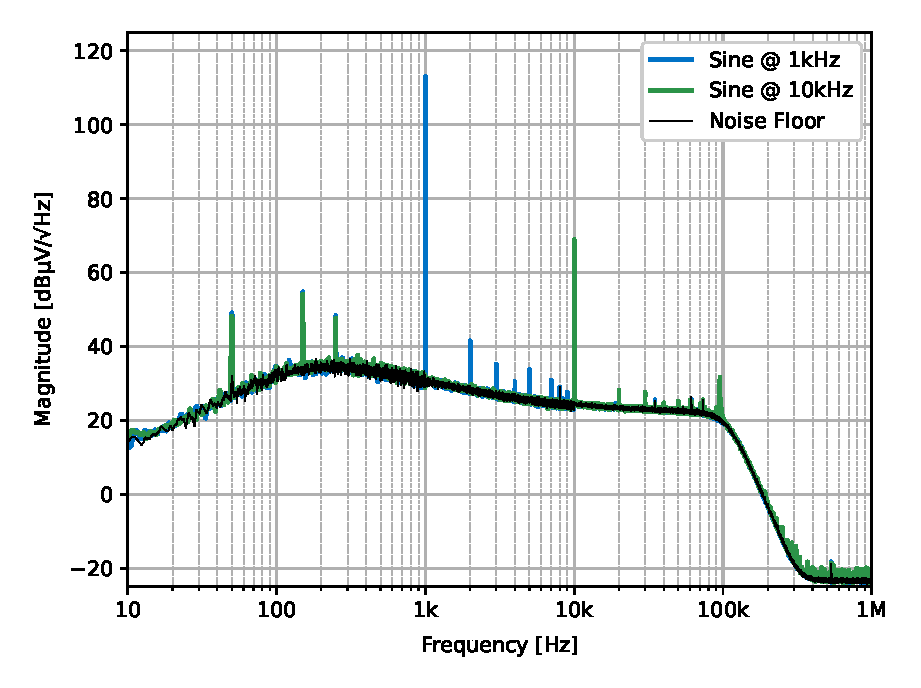
\includegraphics[width=.475\textwidth]{figs/harmonics.eps}
    \caption{Magnetic field measurements.}
    \label{fig:harmonics}
\end{figure}

The results of the harmonic performance analysis, shown in Figure \ref{fig:harmonics}, demonstrated impressive attenuation of approximately $\mathrm{70~dB}$ between the 2\textsuperscript{nd} and 1\textsuperscript{st} harmonics at a fundamental frequency of $\mathrm{1~kHz}$. This high level of attenuation ensures precise signal reproduction and minimal distortion. Although the attenuation was slightly lower at $\mathrm{10~kHz}$ due to the frequency response characteristics of the coil driver, the system effectively suppressed undesired harmonic components, preserving signal integrity.

% --- Noise ---

The ultra-low noise interface circuitry plays a crucial role in enhancing the performance of MR sensors used in the cytometer platform. By minimizing noise-induced fluctuations, the accuracy of magnetic field measurements is preserved, ensuring precise detection of magnetic field changes. The interface circuitry effectively mitigates noise contributions from various sources, including biasing, addressing, amplification, and output multiplexing. Through careful design and optimization, the SNR is improved, leading to enhanced accuracy and reliability of measurements. The noise reduction achieved in this work surpasses the previous interface version, as depicted in Figure \ref{fig:noise}, even with the introduction of additional features such as sensor addressing and output multiplexing. The successful implementation of a different type of reference in the new platform contributed to superior noise performance.

\begin{figure}[!ht]
    \centering
    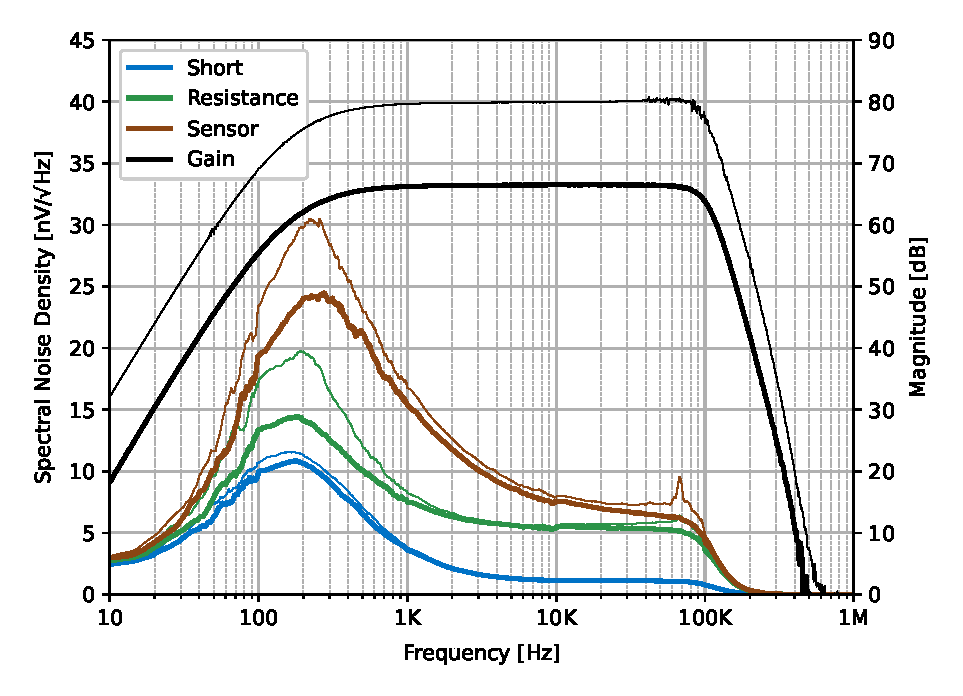
\includegraphics[width=.475\textwidth]{figs/noise.eps}
    \caption{Noise measurements -- Comparison between the old platform and the one presented in this work.}
    \label{fig:noise}
\end{figure}

Figure \ref{fig:noise} displays the noise measurements for both platforms. The thicker line represents the interface developed in this work, while the thinner line represents the previous interface. The graph clearly shows a reduction in overall flicker noise in the new interface. Additionally, the gain has been decreased to accommodate the input voltage limitation of the ADCs.

Overall, the strategies and circuitry optimizations employed in the interface circuitry have resulted in a more robust and reliable system, enabling accurate measurements in the presence of external noise sources.

\begin{figure*}[!htbp]
    \centering
    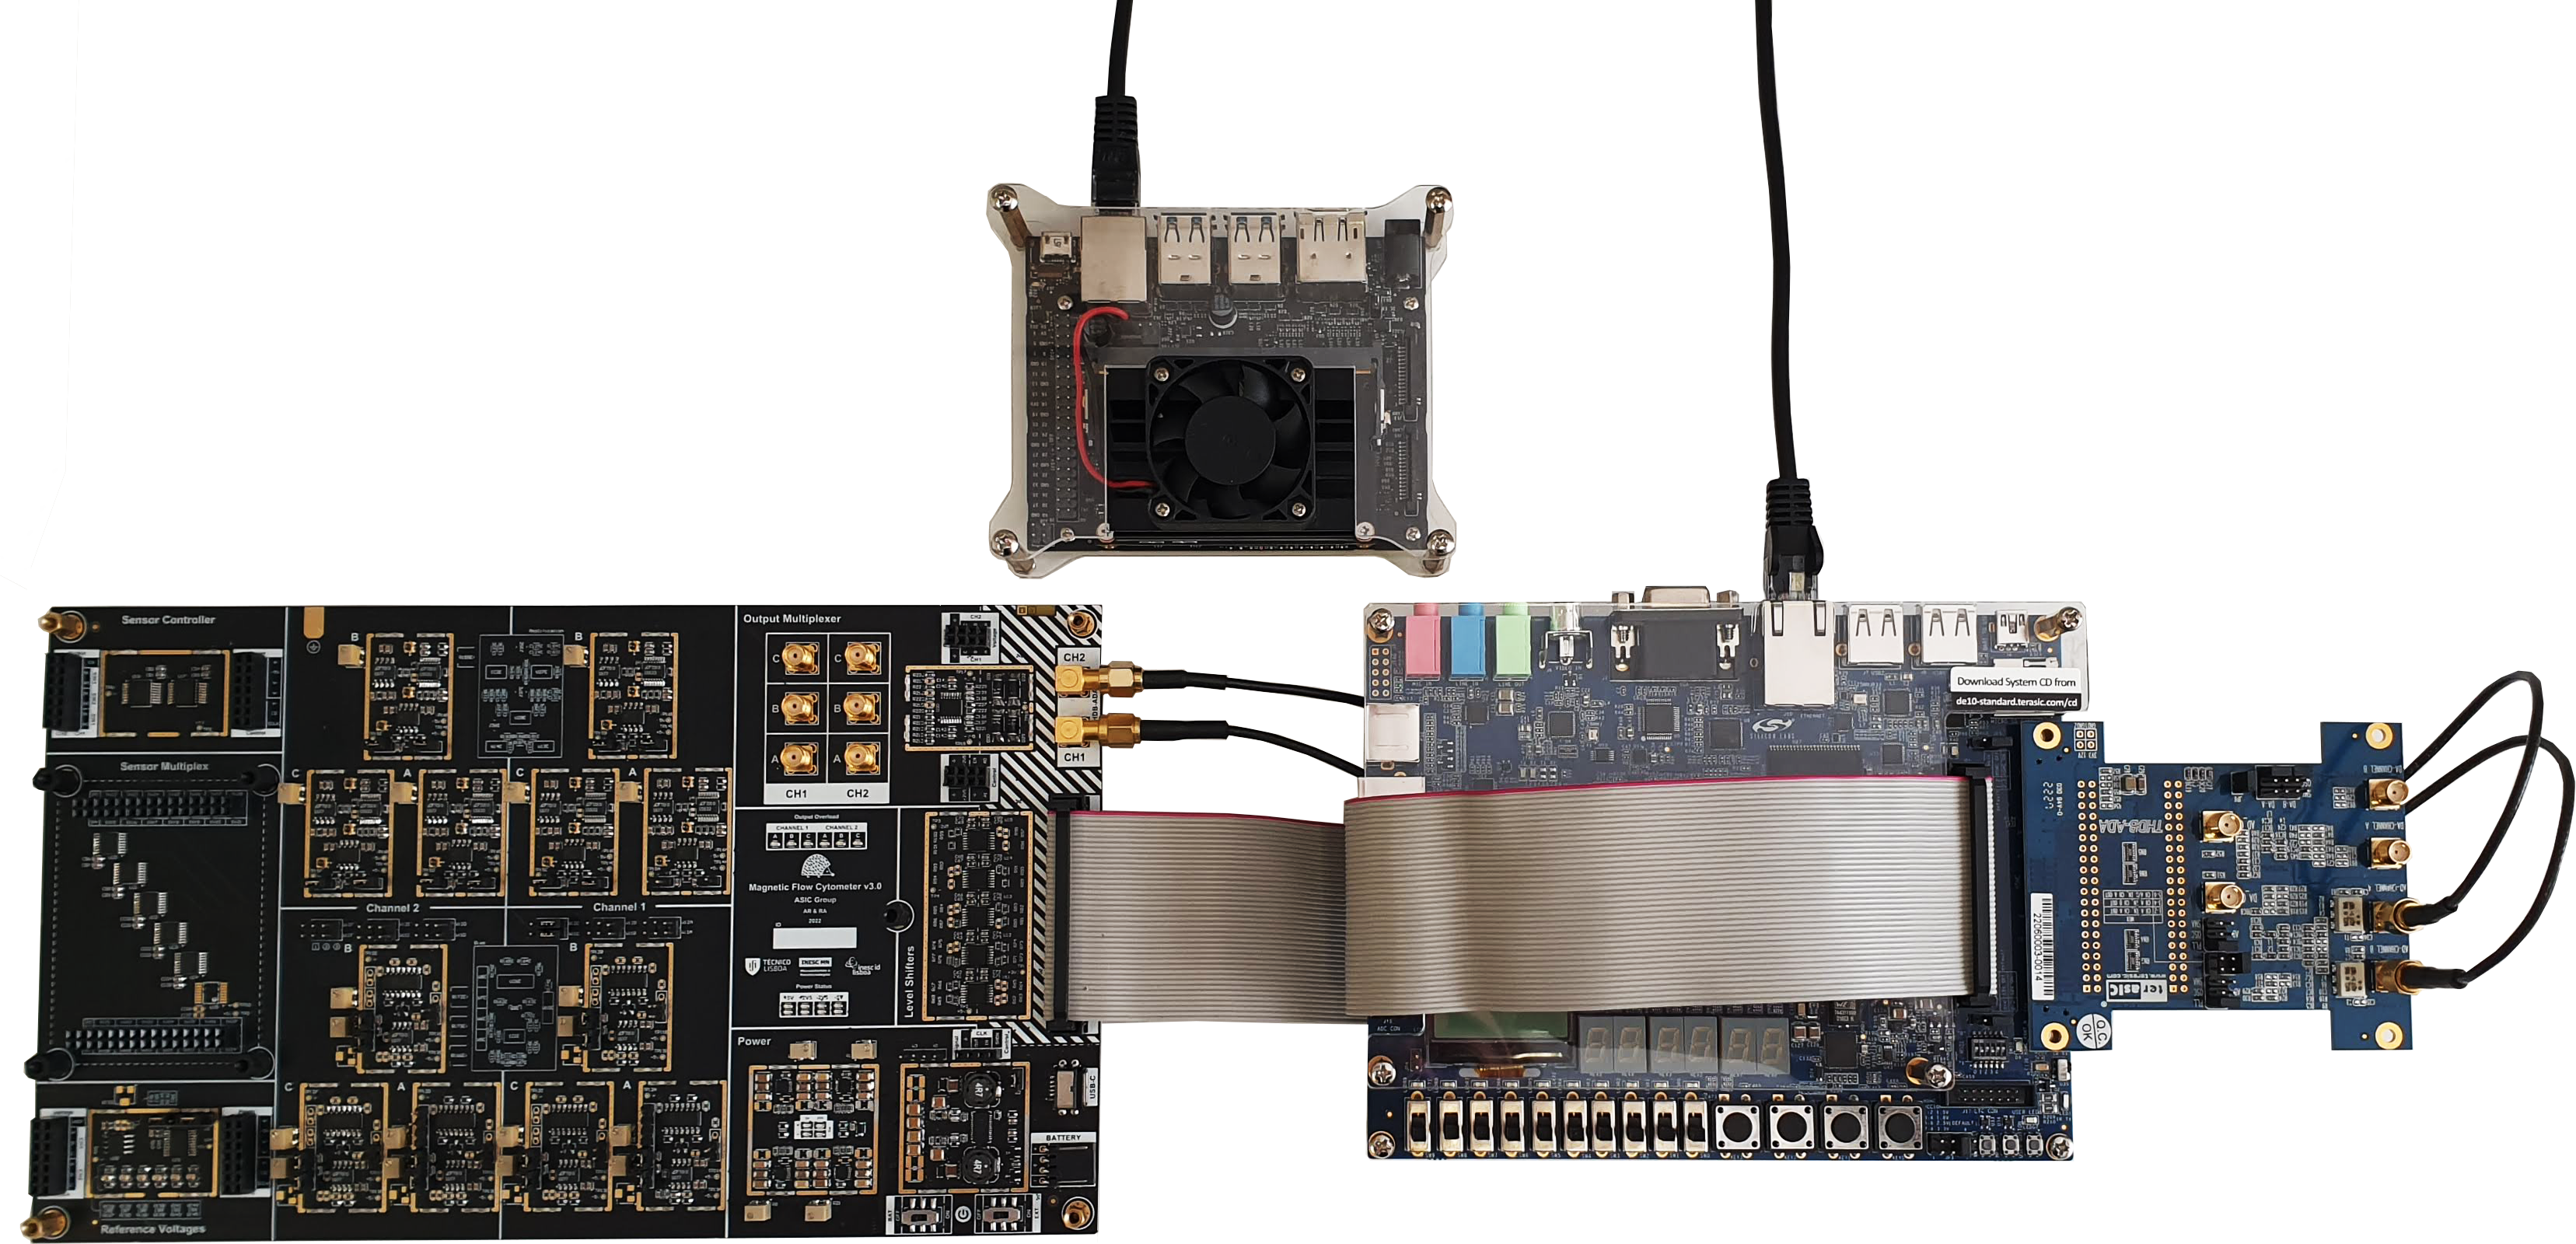
\includegraphics[width=.9\textwidth]{figs/system.png}
    \caption{MFC System.}
    \label{fig:mfc}
\end{figure*}

Figure \ref{fig:mfc} shows the different boards that make up the cytometer system. The left PCB, distinguished by its black solder mask, represents the cytometer platform that was developed as part of the work being described. On the right side, the blue PCB represents the FPGA (DE-10 Standard) and the acquisition board (THDB-ADA). At the top of the figure, the compact computer (Jetson-Nano) serves as the platform that will execute a real-time machine-learning algorithm.
	\section{Conclusions}
\label{sec:concl}

The research conducted in this dissertation focuses on the development of a discrete electronics system for interfacing MR sensors, with a specific emphasis on meeting the requirements for early cancer diagnosis applications. To address the challenges associated with noise propagation and system degradation, an ultra-low noise interface was developed. The architecture underwent significant changes, including modifications to the biasing topology and the incorporation of a flexible reference voltage control. The effectiveness of different sensor placement within the feedback loop was explored, providing alternative configurations for noise reduction. Additionally, improvements were made to the amplification scheme and saturation detection circuitry. The integration of a new circuit allowed for enhanced sensor selection and utilization. Compatibility with the larger MFC system was achieved through supplementary circuits and the implementation of gain reduction multiplexing and level shifters. The power supply configuration was redesigned to meet increased power demands and offer expanded power source options. These advancements lay the groundwork for further progress in MR sensor interfacing and contribute to the development of a robust platform for early cancer diagnosis and related applications.

% REFERENCES

% Produces the bibliography section when processed by BibTeX
%
% Bibliography style
% > entries ordered alphabetically
%\bibliographystyle{plain}
% > unsorted with entries appearing in the order in which the citations appear.
\bibliographystyle{unsrt}
% > entries ordered alphabetically, with first names and names of journals and months abbreviated
%\bibliographystyle{abbrv}
% > entries ordered alphabetically, with reference markers based on authors' initials and publication year
%\bibliographystyle{alpha}

% External bibliography database file in the BibTeX format (ExtendedAbstract_ref_db.bib)
\bibliography{references}

\end{document}


